\begin{table}[!hbt]
	\centering
	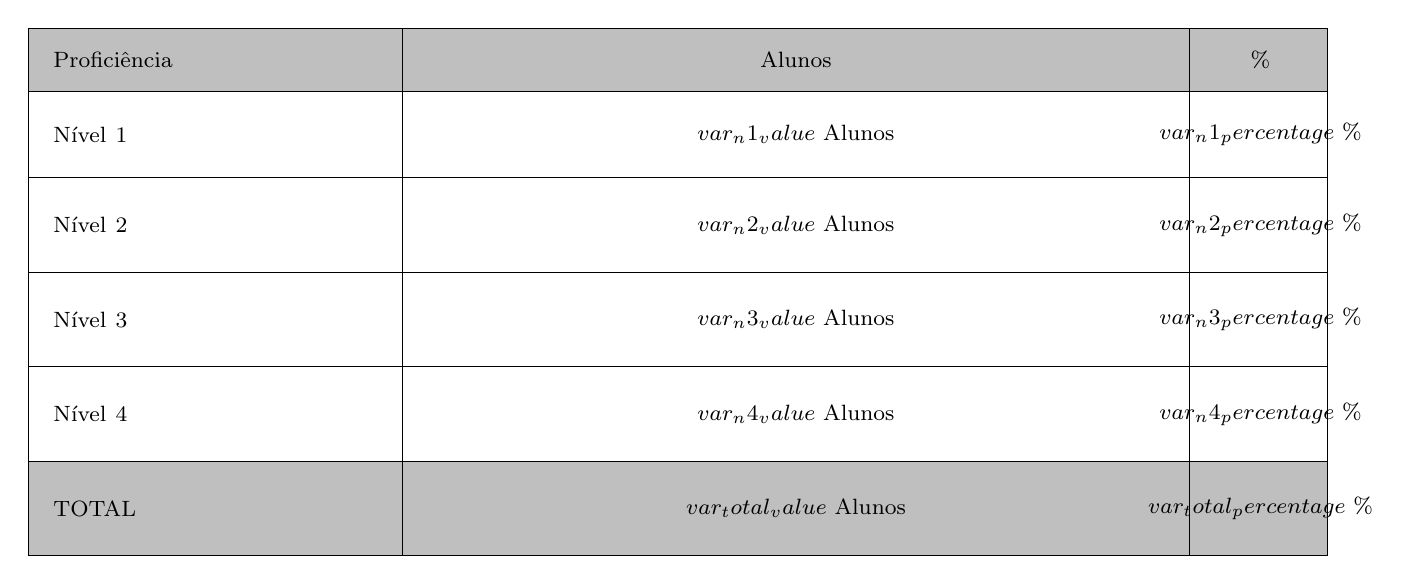
\begin{tikzpicture}
		\fill[lightgray] (-8.25,0.5) rectangle (8.25,-0.3);
		\fill[lightgray] (-8.25,-5) rectangle (8.25,-6.2);
		\draw (-8.25,0.5) rectangle (8.25,-6.2);
		\draw (-8.25,-0.3) -- (8.25,-0.3);
		\draw (-8.25,-1.4) -- (8.25,-1.4);
		\draw (-8.25,-2.6) -- (8.25,-2.6);
		\draw (-8.25,-3.8) -- (8.25,-3.8);
		\draw (-8.25,-5) -- (8.25,-5);

		\draw (-3.5,0.5) -- (-3.5,-6.2);
		\draw (6.5,0.5) -- (6.5,-6.2);

		\node[text width=6cm] at (-4.93,0.1) {\fontsize{8}{0}\selectfont Proficiência};
		\node[text width=6cm] at (-4.93,-0.85) {\fontsize{8}{0}\selectfont Nível 1};
		\node[text width=6cm] at (-4.93,-2) {\fontsize{8}{0}\selectfont Nível 2};
		\node[text width=6cm] at (-4.93,-3.2) {\fontsize{8}{0}\selectfont Nível 3};
		\node[text width=6cm] at (-4.93,-4.4) {\fontsize{8}{0}\selectfont Nível 4};
		\node[text width=6cm] at (-4.93,-5.6) {\fontsize{8}{0}\selectfont TOTAL};

		\node at (1.5,0.1) {\fontsize{8}{0}\selectfont Alunos};
		\node at (1.5,-0.85) {\fontsize{8}{0}\selectfont $var_n1_value$ Alunos};
		\node at (1.5,-2) {\fontsize{8}{0}\selectfont $var_n2_value$ Alunos};
		\node at (1.5,-3.2) {\fontsize{8}{0}\selectfont $var_n3_value$ Alunos};
		\node at (1.5,-4.4) {\fontsize{8}{0}\selectfont $var_n4_value$ Alunos};
		\node at (1.5,-5.6) {\fontsize{8}{0}\selectfont $var_total_value$ Alunos};

		\node at (7.4,0.1) {\fontsize{8}{0}\selectfont \%};
		\node at (7.4,-0.85) {\fontsize{8}{0}\selectfont $var_n1_percentage$ \%};
		\node at (7.4,-2) {\fontsize{8}{0}\selectfont $var_n2_percentage$ \%};
		\node at (7.4,-3.2) {\fontsize{8}{0}\selectfont $var_n3_percentage$ \%};
		\node at (7.4,-4.4) {\fontsize{8}{0}\selectfont $var_n4_percentage$ \%};
		\node at (7.4,-5.6) {\fontsize{8}{0}\selectfont $var_total_percentage$ \%};
	\end{tikzpicture}
\end{table}